% !TEX program = xelatex
\documentclass[10pt,usenames,dvipsnames]{beamer}
\usefonttheme{serif}
\usefonttheme{structuresmallcapsserif}
\usetheme{Madrid}
\usecolortheme{orchid}
\definecolor{royalblue}{RGB}{65,105,225}
\setbeamercolor{structure}{fg=royalblue}
\setbeamercolor{title}{fg=white}
\setbeamercolor{frametitle}{fg=white, bg=royalblue!80!black}
\setbeamercolor{section title}{fg=royalblue!80!black}
\setbeamercolor{subsection title}{fg=royalblue!80!black}
\setbeamercolor{item}{fg=royalblue}
\setbeamercolor{block title}{bg=royalblue!25, fg=royalblue!90!black}
\setbeamercolor{block body}{bg=royalblue!10}
\setbeamercolor{alerted text}{fg=red!80!black}
\setbeamertemplate{blocks}[rounded][shadow=true]
\setbeamertemplate{headline}{} % This line removes the headline template
\usepackage{xcolor}
\beamertemplatenavigationsymbolsempty
\usepackage{tikz}
\usepackage{pgfplots}
\renewcommand{\qed}{\hfill\blacksquare}
\newcommand{\D}[1]{\Delta #1}
\renewcommand{\a}{\alpha}
\usepackage{float}
\setbeamertemplate{frametitle continuation}{%
    \ifnum\insertcontinuationcount>999999999 % this command tells the program when to start counting and also the count will be in numbers and not in roman letters
    \insertcontinuationcount
    \fi}
% ============================================================ %
% HEBREW support via polyglossia %
% ============================================================ %
\usepackage{polyglossia}
\defaultfontfeatures{Mapping=tex-text, Scale=MatchLowercase}
\setdefaultlanguage{hebrew}
\setotherlanguage{english}
\newfontfamily\hebrewfont[Script=Hebrew]{David CLM}
% Use \begin{hebrew} block of text \end{hebrew} for paragraphs.
% Use \texthebrew{ } and \textenglish{ } for short texts.
% ============================================================ %
\title[]{משק פתוח שע''ח נייד}
\author{מתן לבינטוב}
\institute[{{ אב"ג}}]{{ אוניברסיטת בן גוריון בנגב}}
\date{}
\usepackage{bidi}
\begin{document}
\begin{RTL}
\begin{frame}
\titlepage
\end{frame}
\begin{frame}[allowframebreaks]
    \frametitle{שע''ח נייד}
    כאשר המחירים קבועים ושע''ח נייד העוגן הוא כמות הכסף $\left(\frac{M}{P}\right)^S$, כלומר עוקמת $LM$ אינה זזה (כמובן זה בהנחה שלא נעשה שינוי יזום בכמות הכסף).
    \begin{block}{על מה משפיע שע''ח ?}
        כיוון שע''ח משתנה באופן תדיר בתוך המודל, תמיד מאזן התשלומים מתאזן (כלומר נהיה על עקומת $BP$) \\
        כדי להימנע מהזזות מרובות על הגרף, אפשר לאחד את $IS$ ו $BP$ ולהשתמש בעקומת $ISBP$.
    \end{block}


    \framebreak

    \begin{block}{$ISBP$}
        עקומת $ISBP$ היא אוסף נקודות החיתוך בין $IS$ ל $BP$
        $$ISBP : Y = C + I + G  - \underbrace{CF - TR}_{+NX}$$
        $$ISBP : Y =  \frac{1}{1-c} \left[A_0 - TR_0 - CF_0 + cf \times i^* - \left(b+cf \ \right)i \ \right]$$
    \end{block}
    \begin{exampleblock}{יתרון העקומה}
        אינה מושפעת משע''ח 
    \end{exampleblock}
    \begin{alertblock}{חיסרון העקומה}
        לא ניתן לראות בגרף את עודף הביקוש / היצע בשוק המט''ח
    \end{alertblock}    
\end{frame}
\begin{frame}[allowframebreaks]
    \frametitle{תכונות עקומת $ISBP$}
    \begin{itemize}
        \item עקומת $ISBP$ מתונה יותר מ $IS$ : שיפוע $IS$ הוא $\frac{1-c+im}{b}$ לעומת שיפוע $ISBP$ שהוא $\frac{1-c}{b + cf}$
        \item עקומת $ISBP$ שימושית בשע''ח נייד ובשע''ח קבוע ללא עיקור
        \item ש''מ של טווח קצר $LM = ISBP$
        \item $ISBP$ מושפעת מהגדלים הבאים $\left[C_0, G_0, I_0, TR_0 , CF_0, i^{\ *}  \right]$
    \end{itemize}

    

\end{frame}

\begin{frame}
    \frametitle{מצבי קיצון ב $ISBP$}
    \begin{block}{$cf = 0$ סגור לתנועות הון}
        כלומר המשק סגור לתנועות הון ולכן שיפוע העקומה שווה לשיפוע של $IS$ במשק סגור.
        
    \end{block}

    \begin{block}{$cf \to \infty$ תנועות הון מושלמות}
        שיפוע העקומה שווה לשיפוע של $BP$ (גמיש לחלוטין).
    \end{block}

    

\end{frame}
\begin{frame}
    \frametitle{$ISBP$}
    \begin{tikzpicture}[scale=1.2]
        % Axes
        \draw[thick,->] (0,0) -- (7,0) node[right] {$Y$};
        \draw[thick,->] (0,0) -- (0,5) node[above] {$i$};
    
        % Lines
        \draw[thick] (0.5,4.5) -- (4.5,0.5) node[right] {$ISBP$};
        \draw[thick] (0.5,0.5) -- (4.5,4.5) node[right] {$LM$};
        \draw[thick, blue] (1.5,4.5) -- (5.5,0.5) node[right] {$ISBP$};

    
        % Intersection point
        \filldraw [black] (2.5,2.5) circle (2pt) node[above] {A};
        \filldraw [blue] (3,3) circle (2pt) node[above] {C};

    \end{tikzpicture}
    
    

\end{frame}
\begin{frame}
    \frametitle{$IS-BP-LM$}
    \begin{figure}
        \centering
        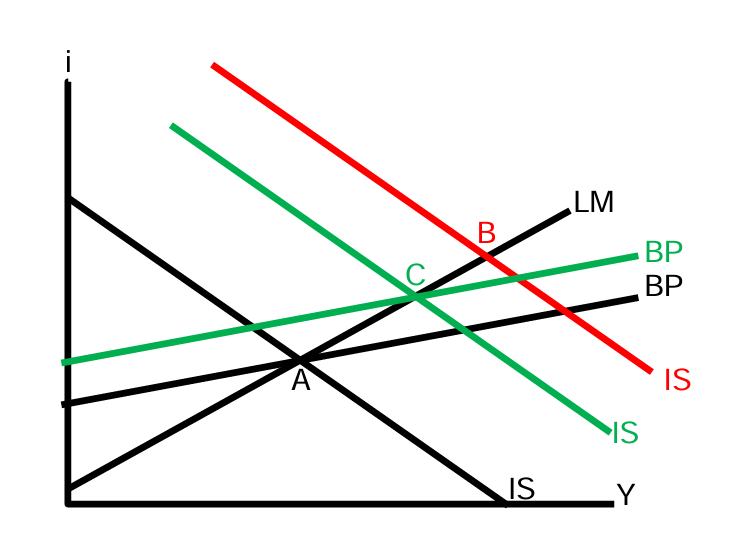
\includegraphics[scale=0.5]{SCR-20240629-nlra.png}
        \caption{השפעת שינוי בשיעור הצריכה על עקומת $ISBP$}
    \end{figure}
    

\end{frame}
\end{RTL}
\end{document}